\section{고속 푸리에 변환 (FFT)}

\begin{frame}
    \frametitle{고속 푸리에 변환}
    \begin{itemize}
        \setlength{\itemsep}{1em}
        \item DFT\,는 그냥 계산하면 \(\O(n^2)\)\,이 소요됨 \pause
        \item \(\omega_n^2 = \omega_{n/2}\) \(\rightarrow\) 분할 정복을 시도!
    \end{itemize}
\end{frame}

\begin{frame}
    \frametitle{고속 푸리에 변환}
    이 절에서는 \(n = 2^k\) (\(k\): 정수) 임을 가정합니다.

    \pause

    \begin{block}{\textbf{Fast Fourier Transform}}
        \(f(x) = a_0 + a_1 x + a_2 x^2 + \cdots + a_{n-1} x^{n - 1}\)\,에 대하여
        \begin{itemize}
            \item \alert{짝수} 차수 항의 계수를 모은 다항식
                  \vspace*{-10px}
                  \[
                      f_{\mathrm{even}} = a_0 + a_2 x + a_4 x^2 + \cdots + a_{n-2} x^{n/2 - 1}
                  \]
                  \vspace*{-30px}
            \item \alert{홀수} 차수 항의 계수를 모은 다항식
                  \vspace*{-10px}
                  \[
                      f_{\mathrm{odd}} = a_1 + a_3 x + a_5 x^2 + \cdots + a_{n-1} x^{n/2 - 1}
                  \]
                  \vspace*{-20px}
        \end{itemize}
        을 생각합니다. \pause 그러면 다음이 성립합니다.
        \vspace*{-5px}
        \begin{center}
            \alert{\(f(x) = f_{\mathrm{even}}(x^2) + x f_{\mathrm{odd}}(x^2)\)}
        \end{center}
        \vspace*{3px}
    \end{block}
\end{frame}

\begin{frame}
    \begin{block}{\textbf{Fast Fourier Transform} (continued)}
        \(\DFT(f)\)\,를 계산하려면, \(f(\omega_{n}^i)\)\,를 계산해야 합니다.
        \[
            f(\omega_{n}^i) = f_{\mathrm{even}}(\omega_{n}^{\alert{2}i}) + \omega_n^i f_{\mathrm{odd}}(\omega_{n}^{\alert{2}i})
        \]
        이고, \pause \(\omega_n^{\alert{2}} = \omega_{n/\alert{2}}\) 이므로
        \[
            f(\omega_{n}^i) = f_{\mathrm{even}}(\omega_{n/\alert{2}}^{i}) + \omega_n^i f_{\mathrm{odd}}(\omega_{n/\alert{2}}^{i})
        \]
        입니다. \pause 한편 \(i = 0,\, 1,\, \dots,\, n - 1\) 인데,
        \[\omega_{n/2}^{i + n/2} = \omega_{n/2}^i \cdot \omega_{n/2}^{n/2} = \omega_{n/2}^i\]
        이므로 사실상 \alert{절반이 겹칩니다!}
    \end{block}
\end{frame}

\begin{frame}
    \begin{block}{\textbf{Fast Fourier Transform} (continued)}
        결국 \(\DFT(f)\)\,를 계산하기 위해서는 \pause
        \begin{itemize}
            \item \(\DFT(f_{\mathrm{even}})\) 계산 \pause
            \item \(\DFT(f_{\mathrm{odd}})\) 계산 \pause
            \item 계산 결과 합치기
        \end{itemize}
        의 과정으로 충분합니다.

        \pause

        \vspace*{10px}

        그런데 \(f_{\mathrm{even}}\), \(f_{\mathrm{odd}}\)\,는 항이 \alert{\(n/2\)}\,개 이므로 이 알고리즘의 시간 복잡도는
        \[
            T(n) = 2T\left(\frac{n}{2}\right) + \O(n) \implies T(n) \in \alert{\O(n\log n)}
        \]
        입니다.
    \end{block}
\end{frame}

\begin{frame}[fragile]
    \frametitle{FFT 구현} \small
    \[
        f(\omega_n^{i}) = \begin{cases}
            f_{\mathrm{even}}(\omega_{n/2}^i) + \omega_{n}^i f_{\mathrm{odd}}(\omega_{n/2}^i) & \text{for } i = 0,\, 1,\, \dots,\, \dfrac{n}{2} \\
            f_{\mathrm{even}}(\omega_{n/2}^i) - \omega_{n}^i f_{\mathrm{odd}}(\omega_{n/2}^i) & \text{for } i = \dfrac{n}{2},\, \dots,\, n - 1
        \end{cases}
    \]

    \begin{lstlisting}[language=Python]
    # Assuming len(f) is a power of 2
    def fft(f: List[complex]) -> List[complex]:
        n = len(f)
        if n <= 1:
            return f

        f_even, f_odd = f[::2], f[1::2]
        fft_even, fft_odd = fft(f_even), fft(f_odd)

        result = [0] * n
        for i in range(n // 2):
            omega = complex(cos(2 * pi / n), sin(2 * pi / n)) ** i

            result[i] = fft_even[i] + omega * fft_odd[i]
            result[i + n // 2] = fft_even[i] - omega * fft_odd[i]

        return result
\end{lstlisting}
\end{frame}

\begin{frame}[fragile]
    \frametitle{Inverse FFT 구현} \small
    Inverse FFT 또한 \(\O(n \log n)\)\,에 수행 가능:
    \begin{itemize}
        \item \(\omega_n^i\)\,만 \(\omega_n^{-i}\)\,로 바뀜
        \item 마지막에 \(1/n\) 해줘야 함
    \end{itemize}

    \begin{lstlisting}[language=Python]
    # Assuming len(f) is a power of 2
    def inverse_fft(f: List[complex]) -> List[complex]:
        n = len(f)
        if n <= 1:
            return f

        f_even, f_odd = f[::2], f[1::2]
        inverse_fft_even, inverse_fft_odd = inverse_fft(f_even), inverse_fft(f_odd)

        result = [0] * n
        for i in range(n // 2):
            omega = complex(cos(2 * pi / n), sin(2 * pi / n)) ** -i

            result[i] = inverse_fft_even[i] + omega * inverse_fft_odd[i]
            result[i + n // 2] = inverse_fft_even[i] - omega * inverse_fft_odd[i]

        return [result_i / 2 for result_i in result]
\end{lstlisting}
\end{frame}

\subsection{곱셈 in \texorpdfstring{\(\O(n \log n)\)}{O(nlogn)}}

\begin{frame}
    \frametitle{다항식의 곱셈 in \(\O(n\log n)\)}
    \begin{center}
        \begin{tikzpicture}[scale=0.6]
            \node (f and g) at (-6, 4) {\(f,\, g\)};
            \node (fg) at (6, 4) {\(fg\)};

            \draw[white,->,thick] (f and g) -- (fg) node[midway,above] {direct multiplication} node[midway,below] {\(\O(n^2)\)};
            \node[white] (dft) at (-6, -4) {\(\DFT(f),\, \DFT(g)\)};
            \draw[white,->,thick] (f and g) -- (dft) node[midway,left] {\(\DFT\)} node[midway,right] {\(\O(n\log n)\)};
            \node[white] (dftf_dftg) at (6, -4) {\(\DFT(f)\cdot\DFT(g)\)};
            \draw[white,->,thick] (dft) -- (dftf_dftg) node[midway,below] {dot product} node[midway,above] {\(\O(n)\)};
            \draw[white,->,thick] (dftf_dftg) -- (fg) node[midway,right] {\(\DFT\inv\)} node[midway,left] {\(\O(n\log n)\)};

            \only<2->{
                \draw[->,thick] (f and g) -- (fg) node[midway,above] {direct multiplication} node[midway,below] {\(\O(n^2)\)};
            }

            \only<3->{
                \node (dft) at (-6, -4) {\(\DFT(f),\, \DFT(g)\)};
                \draw[->,thick,red] (f and g) -- (dft) node[midway,left] {\(\DFT\)} node[midway,right] {\(\O(n\log n)\)};
            }

            \only<4->{
                \node (dftf_dftg) at (6, -4) {\(\DFT(f)\cdot\DFT(g)\)};
                \draw[->,thick,red] (dft) -- (dftf_dftg) node[midway,below] {dot product} node[midway,above] {\(\O(n)\)};
            }

            \only<5->{
                \draw[->,thick,red] (dftf_dftg) -- (fg) node[midway,right] {\(\DFT\inv\)} node[midway,left] {\(\O(n\log n)\)};
            }
        \end{tikzpicture}
    \end{center}
\end{frame}

\subsection{나눗셈 in \texorpdfstring{\(\O(n \log n)\)}{O(nlogn)}}

\begin{frame}
    \frametitle{다항식의 나눗셈 in \(\O(n\log n)\)}
    \begin{itemize}
        \item<1-> \textit{나눗셈은 역수의 곱셉!} \pause \alert{이라고 할 뻔!}\footnote<2->{Ring\,은 나눗셈을 보장하지 않습니다}
    \end{itemize}

    \pause

    \begin{block}{다항식의 나눗셈}
        다항식 \(A(x)\), \(B(x)\)\,에 대하여
        \[
            A(x) = B(x)Q(x) + R(x)
        \]
        인 다항식 \(Q(x)\)\,와 \(\deg R < \deg B\)\,인 다항식 \(R(x)\)\,가 유일하게 존재한다.

        이 때 \(Q(x)\)\,를 \alert{몫}, \(R(x)\)\,를 \alert{나머지}라고 한다.
    \end{block}
\end{frame}

\begin{frame}
    \begin{itemize}
        \setlength{\itemsep}{0.8em}
        \item \(\deg A = n\), \(\deg B = m\)\,이라 하면 \(\deg Q = n - m\)\,이므로 \pause
              \begin{itemize}
                  \item \(A(x) = a_0 + a_1 x + a_2 x^2 + \cdots + a_{n} x^{n}\)
                  \item \(B(x) = b_0 + b_1 x + b_2 x^2 + \cdots + b_{m} x^{m}\)
                  \item \(Q(x) = q_0 + q_1 x + q_2 x^2 + \cdots + q_{n - m} x^{n - m}\)
              \end{itemize}
              \pause
        \item 어차피 \(R(x)\)\,의 차수는 \(m = \deg B\)\,를 넘지 않으므로 \(A(x)\)\,의 첫 \(n - m + 1\)\,개의 항에 영향을 줄 수 없음 \pause
        \item \(A = BQ + R\)\,에서 양변의 첫 \(n - m + 1\)개 항 계수를 비교
              \[
                  \begin{bmatrix}
                      a_n \\ a_{n - 1} \\ \vdots \\ a_{m + 1} \\ a_m
                  \end{bmatrix} = \begin{bmatrix}
                      b_m       & 0      & \cdots & 0         & 0      \\
                      b_{m - 1} & b_m    & \cdots & 0         & 0      \\
                      \vdots    & \vdots & \ddots & \vdots    & \vdots \\
                      \ast      & \ast   & \cdots & b_m       & 0      \\
                      \ast      & \ast   & \cdots & b_{m - 1} & b_m
                  \end{bmatrix} \begin{bmatrix}
                      q_{n - m} \\ q_{n - m - 1} \\ \vdots \\ q_1 \\ q_0
                  \end{bmatrix}
              \]
    \end{itemize}
\end{frame}

\begin{frame}
    \[\small
        \begin{bmatrix}
            a_n \\ a_{n - 1} \\ \vdots \\ a_{m + 1} \\ a_m
        \end{bmatrix} = \begin{bmatrix}
            b_m       & 0      & \cdots & 0         & 0      \\
            b_{m - 1} & b_m    & \cdots & 0         & 0      \\
            \vdots    & \vdots & \ddots & \vdots    & \vdots \\
            \ast      & \ast   & \cdots & b_m       & 0      \\
            \ast      & \ast   & \cdots & b_{m - 1} & b_m
        \end{bmatrix} \begin{bmatrix}
            q_{n - m} \\ q_{n - m - 1} \\ \vdots \\ q_1 \\ q_0
        \end{bmatrix}
    \]
    \begin{itemize}
        \setlength{\itemsep}{0.8em}
        \item 구하는 것은 \(Q(x)\)\,이므로 역행렬을 계산해도 되지만...
        \item<2-> Reversed Polynomial\,을 도입 (다항식 계수 뒤집기!)
              \begin{itemize}
                  \item \(A_R(x) = x^n A(x\inv) = a_n + a_{n - 1} x + \cdots + a_0 x^n\)
                  \item \(B_R(x) = x^m B(x\inv) = b_m + b_{m - 1} x + \cdots + b_0 x^m\)
                  \item \(Q_R(x) = x^{n - m} Q(x\inv) = q_{n - m} + q_{n - m - 1} x + \cdots + q_0 x^{n - m}\)
              \end{itemize} \pause
        \item<4-> 그러면 위 연립방정식은 다음과 같다!
              \[
                  A_R(x) \equiv B_R(x) Q_R(x) \pmod{x^{n - m + 1}}
              \]
    \end{itemize}
\end{frame}

\begin{frame}
    \begin{theorem}[다항식의 나눗셈]
        다항식 \(A(x)\)\,를 다항식 \(B(x)\)\,로 나눈 몫과 나머지 \(Q(x)\), \(R(x)\)\,에 대하여
        \begin{center}
            \(Q_R(x) \equiv A_R(x)\left(B_R(x)\right)\inv \pmod{x^{n - m + 1}}\)
        \end{center}
        이 성립하고 이로부터 \(Q(x)\)\,를 얻을 수 있다. \pause 이제
        \[
            R(x) = A(x) - B(x)Q(x)
        \]
        를 이용해 나머지를 계산할 수 있다.
    \end{theorem}

    \pause

    \begin{itemize}
        \item 다항식의 곱셈, \(\mathrm{mod}\;x^k\)\,에 대한 역원도 \(\O(n\log n)\)\,에 계산 가능 \pause \\
              \(\rightarrow\) \alert{다항식의 나눗셈은 \(\O(n\log n)\)}
    \end{itemize}
\end{frame}

\begin{frame}
    \frametitle{다항식의 \(\mathrm{mod}\;x^k\)\,에 대한 역원}
    \(x\)\,의 역원은...? \pause
    \medskip
    \begin{itemize}
        \setlength{\itemsep}{0.8em}
        \item \(x\)\,와 \(\dfrac{1}{x}\)\,을 곱하면 \(1\) 이지만 \(\dfrac{1}{x}\)\,는 \alert{다항식이 아니다!} \pause
        \item \(\dfrac{1}{x}\)\,을 다항식으로 만드는 방법... \textit{급수 전개}! \pause
        \item<4-> 급수 전개한 뒤 \(\mathrm{mod}\;x^k\)\,를 취한다!
    \end{itemize}

    \pause

    \begin{block}{다항식의 역원}
        다항식 \(f(x)\)\,에 대하여 다음을 만족하는 다항식 \(f(x)\inv\)\,를 찾는다.
        \vspace*{-5px}
        \[
            f(x)\inv f(x) \equiv 1 \pmod{x^k}
        \] \vspace*{-15px}
    \end{block}
\end{frame}

\begin{frame}
    \textit{효율적으로 계산하기 위해서는 먼 길을 돌아갑니다...} \pause
    \begin{itemize}
        \item \(g(x) = f(x)f(-x)\)\,로 정의 \pause
        \item 그러면 \(g(x)\)\,는 우함수이므로 모든 항의 차수가 짝수 \pause
        \item \(g(x) = h(x^2)\)\,으로 두면
    \end{itemize}

    \pause

    \begin{proof}
        \begin{center}
            \(\ds f(x)\inv \equiv \frac{1}{f(x)}\) \pause
            \(\ds \equiv \frac{f(-x)}{f(x)f(-x)}\) \pause
            \(\ds \equiv \frac{f(-x)}{h(x^2)}\) \pause
            \(\ds \equiv f(-x) h(x^2)\inv \pmod{x^k}\)
        \end{center}
    \end{proof}
\end{frame}

\begin{frame}
    \begin{theorem}
        \begin{center}
            \(\ds f(x)\inv \equiv f(-x) h(x^2)\inv \pmod{x^k}\)
        \end{center}
    \end{theorem}

    \pause

    \begin{itemize}
        \setlength{\itemsep}{0.8em}
        \item \(\mathrm{mod}\;x^k\)\,이므로 \(f(x)\)\,의 항은 \(k\)\,개 \pause
        \item \(g(x) = f(x)f(-x)\)\,이므로 항 개수가 2배가 되지만 \(x^k\)\,이상은 버림 \pause
        \item 짝수 차수 항만 남았으므로 \(h(x)\)\,의 항의 개수는 \(f(x)\)\,의 대략 절반 \pause
        \item 재귀적으로 계산: \(h(x^2)\inv \mod{x^k} \rightarrow h(x)\inv \mod{x^{\lfloor k/2 \rfloor}}\)
    \end{itemize}

    \pause

    \vspace*{10px}

    따라서 시간복잡도는
    \[
        T(n) = T\left(\dfrac{n}{2}\right) + \underbrace{\O(n \log n)}_{g,\,h\,\text{계산}} \implies T(n) \in \alert{\O(n \log n)}
    \]
\end{frame}


